%==============================================================================
% Capítulo 6: Implementación
%==============================================================================
\section{Implementación}\label{sec:implementacion}

\subsection{Entorno de despliegue y dependencias}\label{subsec:entorno-despliegue}

La implementación del sistema se llevó a cabo combinando componentes de código abierto ---Python, FastAPI y PostgreSQL--- con N8N, cuya licencia Sustainable Use (\emph{fair-code}) permite auditar su código fuente, con el objetivo de garantizar la portabilidad, la reproducibilidad y la auditoría de seguridad de la solución en organizaciones medianas. Toda la infraestructura se encapsula mediante contenedores Docker, orquestados localmente por Docker Compose para los entornos de desarrollo y preproducción; la migración a un cluster Kubernetes~1.30 para el entorno productivo se plantea como trabajo futuro y no cuenta con manifiestos de despliegue en esta versión (\autoref{sec:recomendaciones}).

Las versiones específicas de los componentes son: N8N~2.11.2, Python~3.12, PostgreSQL~15.5 con volumen persistente, FastAPI~0.115, Uvicorn 0.30.6, SQLAlchemy~2.0, y el cliente google-genai >=2.20.0 (SDK unificado de Google Generative AI) para la comunicación con el modelo \texttt{gemini-3.6-flash}. Todos los servicios se despliegan sobre imágenes Docker oficiales (\texttt{python:3.12-slim} y \texttt{postgres:15.5-alpine}). La gestión de dependencias del módulo Python se realiza mediante un archivo \texttt{requirements.txt} con versiones fijadas (\emph{pinned}) para garantizar la reproducibilidad de las compilaciones en distintos entornos.

\subsection{Construcción del módulo Python}\label{subsec:construccion-modulo-python}

La selección del marco de trabajo para el servicio de procesamiento implicó la evaluación de tres alternativas: Flask, Django REST Framework y FastAPI. Flask, ampliamente adoptado en el ecosistema Python por su simplicidad, carece de validación nativa de esquemas y de generación automática de documentación OpenAPI, funcionalidades que el proyecto requería para garantizar la calidad de la interfaz REST. Django REST Framework, por su parte, ofrece un conjunto completo de herramientas para la construcción de interfaces de programación de aplicaciones, pero su modelo de operación sincrónico y la inclusión de componentes no requeridos por el proyecto ---tales como el ORM de Django y el motor de plantillas--- incrementaban la complejidad de la base de código sin aportar beneficios funcionales para una arquitectura de microservicio acotado. FastAPI~0.115, sustentado sobre el servidor ASGI Uvicorn 0.30.6, ofrece tres ventajas determinantes para el proyecto: validación automática de esquemas de entrada y salida mediante Pydantic~v2, generación de documentación interactiva conforme a la especificación OpenAPI~3.1 sin configuración adicional, y operación asincrónica nativa que permite manejar las llamadas concurrentes desde N8N sin bloquear el hilo de ejecución principal \parencite{Tiangolo2024_fastapi}. La madurez del ecosistema de FastAPI, su adopción creciente en la industria y la disponibilidad de documentación exhaustiva en español consolidaron la decisión.

El módulo Python expone su contrato REST organizado en capas, según la estructura descrita en la \autoref{sec:arquitectura}, con una separación clara entre responsabilidades:

\begin{itemize}
  \item \textbf{models}: entidades del modelo de dominio mapeadas mediante SQLAlchemy~2.0.
  \item \textbf{schemas}: modelos de validación y serialización con Pydantic~v2.
  \item \textbf{services}: lógica de aplicación (IncidenteService, ClasificacionService).
  \item \textbf{repositories}: acceso a datos, aislando las consultas SQL del resto de la aplicación.
  \item \textbf{classifiers}: lógica del clasificador híbrido (filtro determinístico + LLM).
  \item \textbf{routes}: enrutadores REST que delegan en los servicios correspondientes.
  \item \textbf{core}: configuración de base de datos, manejo de errores y logging estructurado.
\end{itemize}

La construcción se realiza bajo un esquema de inyección de dependencias gestionado por las funcionalidades nativas de FastAPI (\texttt{Depends}), lo que facilita el reemplazo de implementaciones durante la ejecución de pruebas unitarias y de integración. Esta arquitectura permite, por ejemplo, sustituir el clasificador real por una implementación simulada durante las pruebas sin modificar el código de los servicios que lo consumen. La gestión de credenciales se realiza exclusivamente mediante variables de entorno, en línea con el principio de configuración de la metodología Twelve-Factor App \parencite{Wiggins2017_12factor}.

\subsection{Construcción del flujo en N8N}\label{subsec:construccion-flujo-n8n}

El flujo de orquestación implementado en N8N comprende 32 nodos (29 operativos más 3 notas adhesivas), organizados en siete etapas funcionales pero con ramificaciones específicas por canal. La elección de N8N como plataforma de orquestación, frente a alternativas como Apache Airflow, Zapier o Make, obedeció a tres criterios concurrentes. El primero, de naturaleza operativa, radica en que N8N admite despliegue completamente autoalojado bajo Docker, manteniendo los flujos de procesamiento y los datos dentro del perímetro organizacional. Zapier y Make operan exclusivamente como servicios en la nube, lo que las descarta en escenarios donde el procesamiento de datos sensibles exige control de infraestructura. Apache Airflow, aunque autoalojable, diseña sus flujos como grafos acíclicos dirigidos programados por intervalos temporales; ese paradigma resulta adecuado para procesos de extracción, transformación y carga de datos pero forzadamente inadecuado para un sistema reactivo que debe responder en tiempo real a eventos de entrada no programados \parencite{Apache2024_airflow}. El segundo criterio refiere al modelo de construcción visual que N8N ofrece sobre un editor de nodos arrastrables: la curva de aprendizaje de esta interfaz es sustancialmente menor que la de alternativas centradas en definición programática de flujos, lo que permitió al equipo concentrar el esfuerzo en la lógica de negocio antes que en la sintaxis de definición de procesos. El tercer criterio se vincula con la licencia de código fuente disponible (\emph{fair-code}) que habilita la auditoría de seguridad del núcleo de orquestación \parencite{n8n2024_docs}.

La composición de los 29 nodos responde a un patrón de procesamiento por canal, de cinco pasos, que se replica para cada medio de ingreso con ramificaciones específicas según el canal:

\begin{enumerate}[leftmargin=*]
  \item \textbf{Recepción}: Tres disparadores (\emph{triggers}) reciben las entradas desde correo electrónico (IMAP), formulario web (Webhook) y telefonía (trigger de Twilio). La decisión de separar los disparadores por canal, en lugar de unificar la recepción mediante un único webhook con discriminación interna, se fundamenta en la necesidad de preservar la configuración de autenticación y los parámetros de reintento específicos de cada protocolo.
  \item \textbf{Normalización}: Un nodo de transformación (\emph{Function}) homogeniza la estructura del mensaje en un formato unificado \parencite{Hohpe2003_eip} con campos de identificador único (UUID v4), marca temporal, canal de origen, remitente y descripción textual normalizada. Esta etapa elimina las diferencias de formato entre canales y garantiza que las capas posteriores procesen siempre la misma estructura de datos, independientemente de la vía de entrada.
  \item \textbf{Clasificación y persistencia}: Un nodo HTTP invoca el endpoint \texttt{POST /api/v1/incidentes} del módulo Python enviando la descripción textual junto con los metadatos del canal. La clasificación no se expone como punto de entrada independiente sino que se encuentra embebida dentro de la creación del incidente: el clasificador híbrido se invoca internamente durante la creación, que persiste el ticket en la misma operación, y la respuesta incluye el identificador del ticket, la categoría asignada y el indicador de revisión humana (\texttt{requiere\_revision\_humana}), que el backend activa según las condiciones descritas en la etapa de evaluación. El canal telefónico no constituye una excepción: su clasificación se resuelve dentro del backend mediante la misma cascada híbrida que los canales escritos, aplicada sobre la descripción pseudonimizada, y el cuerpo de la creación no transporta una clasificación precalculada.
  \item \textbf{Evaluación}: Aguas abajo del POST, un nodo condicional (\emph{IF}) evalúa el indicador de revisión humana devuelto por el backend. Cuando el indicador está activo el flujo notifica al operador designado por correo electrónico y registra el evento en la auditoría; cuando no lo está, el flujo continúa automáticamente con las confirmaciones al usuario. Con anterioridad al POST, un nodo de validación de entrada verifica que la descripción no esté vacía y respete la longitud mínima y máxima aceptada por el backend, de modo que una entrada inválida no genera un incidente. El backend activa el indicador cuando la etapa Gemini devuelve una confianza inferior a 0,70, cuando interviene la etapa de reserva o cuando el reportante no se identifica en el directorio de empleados; los casos que resuelve el filtro determinístico no se derivan por su confianza (\autoref{subsec:subsistema-clasificacion}). La calibración de la confianza del modelo se analiza en la Sección~\ref{subsec:calibracion}.
  \item \textbf{Notificación}: Tres nodos posteriores notifican al usuario por el canal correspondiente y registran la ejecución en el sistema de auditoría; la persistencia del ticket ocurre en el mismo POST de creación, que almacena el incidente y su clasificación en una sola operación. El paralelismo de la notificación garantiza que la demora de un canal (por ejemplo, el envío de correo electrónico) no bloquee el registro de auditoría ni la confirmación por otros medios.
\end{enumerate}

El canal telefónico incorpora un nodo adicional de normalización y validación que prepara la transcripción pseudonimizada antes de incorporarla al flujo principal, pero no determina el sector persistido: la rama de clasificación por agente LLM basada en LangChain fue retirada (decisión OQ1 = A del change c-72). La clasificación del incidente telefónico se rige por el diseño unificado descrito en la \autoref{subsec:subsistema-clasificacion}.

La trazabilidad completa de cada ejecución se preserva almacenando los identificadores de nodo, las marcas temporales de entrada y salida de cada etapa, y los datos de entrada y salida de cada paso del flujo, generando un historial auditable que resulta especialmente valioso en contextos donde la Ley~25.326 exige demostrar el camino recorrido por los datos personales \parencite{Ley25326_2000}. La exportación completa del flujo en formato JSON se incluye en el Anexo~E.

\subsection{Integración del canal telefónico}\label{subsec:integracion-canal-telefonico}

La integración con Twilio se realizó mediante el producto Programmable Voice, complementado con la transcripción automática nativa. El flujo telefónico opera de la siguiente manera: el usuario marca un número virtual asignado a la organización; un script TwiML reproduce un mensaje de bienvenida en español rioplatense y solicita al usuario describir su problema durante un máximo de 45 segundos; la grabación finaliza cuando el usuario presiona la tecla numeral (\texttt{\#}) o transcurrido el tiempo máximo; la grabación se envía al servicio de transcripción de Twilio; y, una vez transcrito el contenido, Twilio invoca un webhook expuesto por N8N con la transcripción textual. A partir de ese punto, el flujo continúa de manera idéntica a la de los canales escritos.

El tiempo de registro del canal telefónico ---medido, para igualar la base de comparación con el flujo manual, desde el inicio de la llamada hasta la confirmación del número de incidente--- promedió 20,1 segundos sobre los 81 casos del corpus. Ese total comprende la duración de la llamada grabada y la latencia de procesamiento posterior al cuelgue; el corpus registra la suma de ambos tramos, no su descomposición por etapa (transcripción, clasificación y persistencia), de modo que no se publica un desglose de latencias que el repositorio no permite reproducir con tamaño de muestra y procedimiento de medición. La grabación está acotada a un máximo de 45~s, de modo que el tiempo telefónico reportado constituye una cota inferior de la duración real de la llamada.

Unificada la clasificación, el canal telefónico dejó de reservar la superficie de costo asociada a la invocación incondicional del agente en N8N. La clasificación pasa a computarse en la superficie de inferencia del backend y solo cuando la cascada híbrida escala al modelo semántico; los casos resueltos por el filtro determinístico no consumen cuota de Gemini. Este traslado de la superficie de costo corresponde a la decisión OQ2 = A del change c-72 y elimina la reserva telefónica del proveedor invocado desde N8N.

\subsection{Desafíos de integración}\label{subsec:desafios-integracion}

La implementación del sistema enfrentó tres desafíos de integración que merecen documentación explícita por su potencial utilidad en replicaciones futuras.

El primer desafío se presentó en la comunicación asincrónica entre N8N y el servicio de clasificación. El nodo HTTP de N8N invoca el endpoint de clasificación de manera sincrónica y espera la respuesta del servidor antes de continuar el flujo. Esta arquitectura, aunque simple de implementar, introduce un punto de fallo único: si el servicio Python no responde dentro del tiempo de espera configurado en el nodo HTTP, el flujo completo se detiene y el incidente queda sin procesar. Esta limitación se asume como conocida en la versión evaluada: no se implementó un mecanismo de reintento con retroceso exponencial ni una cola de respaldo en el servicio Python que retuviera los mensajes durante ventanas de saturación. La disponibilidad ante fallas transitorias del servicio de clasificación queda, por lo tanto, como trabajo futuro, junto con la definición de una política de reintentos idempotente que preserve la trazabilidad de cada intento.

El segundo desafío surgió de la heterogeneidad de los formatos de entrada. Los correos electrónicos incluyen encabezados, firmas corporativas y reenvíos que contaminan el texto que el clasificador recibe; las llamadas telefónicas transcritas introducen errores de reconocimiento del habla, particularmente en términos técnicos (por ejemplo, \texttt{API} transcrito como \texttt{a p i} o \texttt{apeye}); y los formularios web, aunque proveen texto limpio, llegan con una proporción significativa de campos vacíos o con descripciones de una sola palabra. La respuesta a esta heterogeneidad fue doble. Por un lado, se implementó un preprocesador en el nodo de normalización de N8N que elimina firmas, encabezados de reenvío y líneas de disclaimer mediante expresiones regulares específicas del dominio de correo institucional. Por el otro, se enriqueció el prompt enviado al clasificador con instrucciones explícitas para interpretar términos técnicos frecuentemente mal transcritos, lo que mejoró la robustez de la clasificación sobre transcripciones automáticas respecto de la configuración inicial sin estas instrucciones.

El tercer desafío, de naturaleza operativa, se vincula con la persistencia transaccional de la sesión de clasificación. El sistema debe garantizar que una vez que el clasificador asigna una categoría, el incidente se persiste con esa decisión o, en caso de falla de la base de datos, el estado interno del sistema refleje la inconsistencia y pueda recuperarse. La solución adoptó un enfoque pragmático: N8N invoca la creación del incidente ---que clasifica y persiste en una sola operación del backend--- como paso único del flujo. El nodo HTTP de creación declara un enrutamiento de error (\texttt{continueErrorOutput}): ante una falla de persistencia, la ejecución se desvía hacia la rama de error del flujo en lugar de reintentar automáticamente la operación. La recuperación del incidente exige, por lo tanto, una reejecución manual del flujo o el reproceso del mensaje de origen, situación que se asume como limitación conocida de la versión evaluada y se propone como trabajo futuro junto con una política de reintentos idempotente. La tabla de trazabilidad (\texttt{clasificacion\_log}) fue diseñada para admitir múltiples registros de clasificación por incidente, preservando así el historial de cada intento.

\subsection{Conexión con el proceso Scrumban}\label{subsec:conexion-scrumban}

La construcción del sistema fue organizada bajo el esquema Scrumban descrito en la \autoref{sec:marco-metodologico}, ejecutando iteraciones de duración variable, ubicadas sin fechar por separado en los dos períodos de actividad del repositorio (\autoref{fig:cronograma}, Anexo~A). La vinculación entre cada etapa de construcción y los artefactos de implementación producidos se detalla a continuación:

\begin{enumerate}[label=Etapa \arabic*:, leftmargin=*]
  \item La elicitación de requisitos produjo el diseño preliminar de la arquitectura de cinco capas y la especificación de la interfaz REST, documentadas en la \autoref{sec:arquitectura}.
  \item La construcción del módulo Python entregó el modelo de datos, los repositorios con operaciones CRUD asincrónicas y los servicios de negocio. Al cierre de esta etapa, el módulo Python exponía el endpoint de salud y aceptaba la creación de incidentes mediante \texttt{POST /api/v1/incidentes}, con la cobertura de pruebas unitarias medida por pytest-cov sobre los paquetes de rutas, servicios y repositorios (véase la \autoref{subsec:pruebas-automatizadas}).
  \item La configuración inicial del flujo N8N implementó el canal de correo electrónico como vía prioritaria, estableciendo el patrón de procesamiento por canal que luego se replicaría para los canales restantes. Al finalizar esta etapa, el sistema procesaba incidentes por correo electrónico de extremo a extremo, desde la recepción hasta la notificación.
  \item La integración del canal telefónico y la persistencia incorporó Twilio Programmable Voice, el script TwiML y la configuración del webhook de transcripción. Esta etapa fue la que más expuso los desafíos de heterogeneidad de formatos descritos en la \autoref{subsec:desafios-integracion}, y su resolución consumió aproximadamente el 40~\% del esfuerzo de la etapa.
  \item La validación funcional y el ajuste fino del clasificador se concentraron en la calibración del filtro determinístico y del prompt de Gemini. Los ajustes se realizaron a partir de errores observados en el corpus de validación; no se dispuso de un conjunto independiente de incidentes de preproducción (\autoref{subsec:interpretacion-resultados}).
  \item La validación experimental y la documentación final ejecutaron el protocolo de pruebas descrito en la \autoref{sec:marco-metodologico}, recolectaron las mediciones del corpus completo y produjeron el análisis estadístico presentado en la \autoref{sec:resultados}.
\end{enumerate}

La campaña del flujo manual (junio a agosto de 2026) no es una etapa de construcción; la del flujo automatizado (septiembre a octubre de 2026) corresponde a la validación experimental, con \texttt{gemini-3.6-flash} integrado el 24 de septiembre de 2026.

La trazabilidad entre etapas y artefactos, mediada por el tablero Kanban en Jira, permitió al equipo identificar tempranamente los desvíos respecto del plan y redistribuir el esfuerzo cuando la complejidad de un componente superaba la estimación inicial. La adopción de límites de trabajo en curso (WIP) por columna del tablero evitó la acumulación de tareas a medio terminar, una práctica que resultó particularmente valiosa durante las etapas 4 y 5, donde la interdependencia entre módulos exigía finalizar componentes antes de integrarlos.

\subsection{Pruebas automatizadas}\label{subsec:pruebas-automatizadas}

La estrategia de pruebas se sustentó en la pirámide clásica descrita por \textcite{Crispin2009_agile_testing}. En la base se ubicaron las pruebas unitarias del módulo Python construidas con el marco pytest~8.3. La cobertura de código de aplicación se mide con pytest-cov 5.0.0 sobre los paquetes de rutas, servicios y repositorios, mediante el comando \texttt{pytest --cov=app.routes --cov=app.services --cov=app.repositories --cov-report=term-missing}, cuyo reporte se genera en cada ejecución del pipeline de integración continua; la cifra exacta queda sujeta al reporte vigente y no se fija en el texto para no declarar un valor no reproducible. Estas pruebas cubren los clasificadores (determinístico e híbrido), los servicios de negocio, los esquemas de validación y los repositorios de acceso a datos.

En el nivel intermedio se ejecutaron pruebas de integración en dos variantes complementarias: (a)~pruebas rápidas contra SQLite en memoria para la ejecución durante el desarrollo, utilizando el fixture \texttt{db\_session} con rollback por test; y (b)~pruebas de integración contra una instancia real de PostgreSQL~15.5, que validan comportamientos específicos del motor ---integridad de claves foráneas, eliminación en cascada, restricciones UNIQUE, precisión de tipos \texttt{Numeric(5,4)} y zona horaria en \texttt{TIMESTAMPTZ}, índices compuestos y coexistencia de esquemas--- mediante 16 tests con un mecanismo de omisión automática (\texttt{pytest.skip}) cuando PostgreSQL no está disponible. En el nivel superior no se dispone de pruebas de extremo a extremo que instancien N8N y ejecuten el flujo completo: la integración con la plataforma de orquestación se verifica de forma estructural, mediante pruebas que parsean y validan el archivo \texttt{n8n/workflow.json} (composición de nodos, conexiones y límites de costo) y pruebas de API y de base de datos que ejercitan los endpoints y la persistencia del módulo Python. La ejecución del flujo dentro de una instancia N8N activa queda fuera del alcance de la suite automatizada.

El frontend se desarrolló como una aplicación React 19 de página única (SPA) con TypeScript y Vite como herramienta de construcción. La aplicación consta de dos vistas principales: un portal de reporte de incidentes con validación de formularios, y un panel de administración que incluye listado de tickets con filtros combinados, cola de revisión humana para los casos derivados por el backend, y visualización detallada de cada incidente con trazabilidad completa de la decisión del clasificador. La comunicación con el backend se realiza mediante Axios, y la gestión del estado del servidor se apoya en React Query para caching y revalidación automática.

El frontend cuenta con una suite de 357 pruebas automatizadas distribuidas en 56 archivos, construidas con Vitest y Testing Library, que alcanza una cobertura de sentencias del 99,6~\% sobre los paquetes medidos, conforme al reporte reproducido con \texttt{npm run test:coverage}; la cifra queda sujeta al reporte vigente en cada ejecución del pipeline de integración continua.

La integración continua (CI) se ejecuta automáticamente en cada solicitud de incorporación (\emph{pull request}) al repositorio mediante GitHub Actions, ejecutando la suite completa de pruebas unitarias y de integración antes de permitir la fusión a la rama principal. El pipeline de CI incluye verificación de estilo de código (Ruff), ejecución de pruebas con reporte de cobertura, y verificación de sincronización de la especificación OpenAPI.

\subsection{Dashboard de analítica}\label{subsec:dashboard-analitica}

El panel de administración incluye un dashboard de analítica desarrollado con la biblioteca ReCharts de React. Este módulo proporciona visualización agregada de los datos históricos de incidentes, permitiendo identificar tendencias temporales, patrones de fallas recurrentes y desequilibrios en la distribución de carga entre sectores. Esta capacidad de análisis retrospectivo transforma los datos operativos acumulados en inteligencia organizacional accionable. La Figura~\ref{fig:panel_admin} muestra el panel de administración sobre el que se integra esta capacidad analítica, con el listado de tickets, los filtros combinados y la pestaña de revisión humana para los casos derivados por el backend.

\begin{figure}[htbp]
\centering
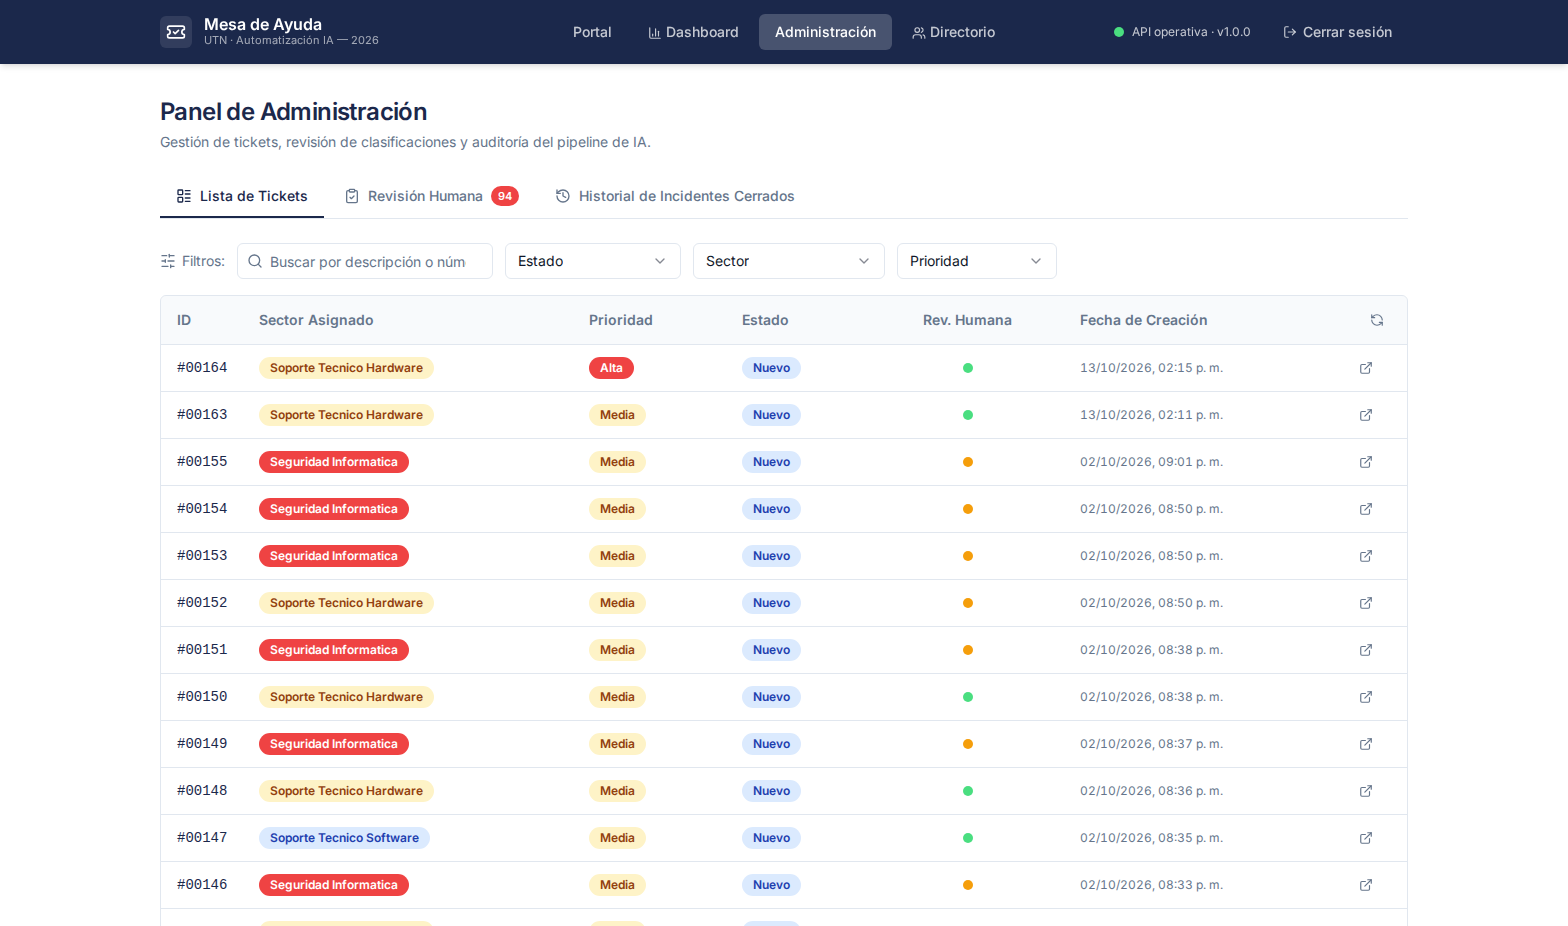
\includegraphics[width=\textwidth]{panel_admin}
\caption{Panel de administración del sistema: listado de tickets con filtros combinados y cola de revisión humana.}
\label{fig:panel_admin}
\end{figure}

El dashboard se organiza en tres visualizaciones principales. Un gráfico de tendencias muestra la evolución temporal de los incidentes, agrupables por día o por mes según la granularidad seleccionada por el operador. Un gráfico de torta presenta la distribución proporcional de incidentes entre los cinco sectores responsables. Un gráfico de barras apiladas desglosa los incidentes según su estado en el ciclo de vida, facilitando la identificación de cuellos de botella en la resolución. La Figura~\ref{fig:dashboard} presenta estas tres visualizaciones junto con los indicadores agregados del período seleccionado.

\begin{figure}[htbp]
\centering
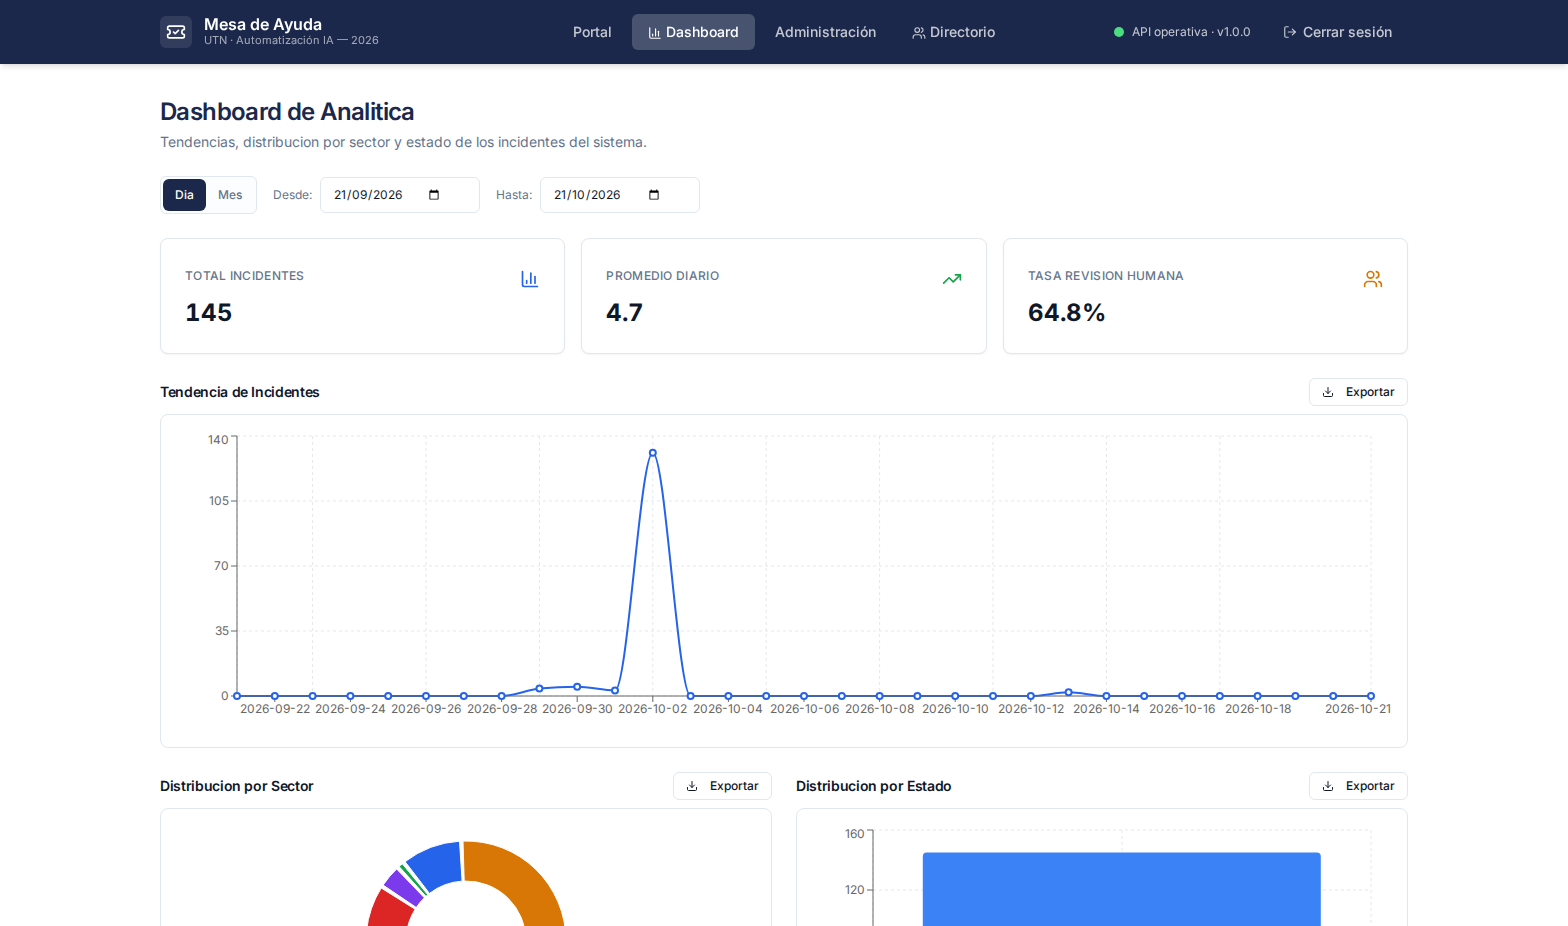
\includegraphics[width=\textwidth]{dashboard}
\caption{Dashboard de analítica del panel de administración: tendencia temporal de incidentes, distribución por sector y distribución por estado.}
\label{fig:dashboard}
\end{figure}

Los controles de filtro permiten acotar el período de análisis mediante un rango de fechas configurable, y alternar entre agrupación diaria y mensual para adaptar la granularidad al horizonte temporal de interés. Cada gráfico puede exportarse como imagen PNG para su inclusión en informes periódicos o presentaciones.

La utilidad práctica del dashboard puede ilustrarse con un escenario hipotético: si el sistema detectara que veinte usuarios reportaron la rotura de auriculares en una franja temporal acotada, el patrón sugeriría un problema de calidad del proveedor antes que una serie de fallas aisladas. Esta capacidad de identificar causas raíz a partir de datos agregados constituye un salto cualitativo respecto del enfoque tradicional de gestión de incidentes, donde cada ticket se trata de forma aislada y los patrones sistémicos permanecen invisibles.

\newpage
